\documentclass[11pt]{article}

\usepackage{pablo}
\usepackage{pablo-listings}
\usepackage{tkz-tab}
\usepackage[a5paper,margin=1.8cm]{geometry}
\usepackage{multicol}

\pagestyle{empty}
\begin{document}

\begin{center}
  {\large
    Devoir surveillé --- Corrigé

    \textsc{Équations --- Repérage}
  }
\end{center}

\begin{exercice}[(In)équations]~
  \begin{enumerate}
    \item \emph{Résoudre l'équation :
      $\dfrac{2+x}{x-3}=0$}

      Cette équation est vraie lorsque $2+x=0$ et $x-3\neq0$ (car on ne peut pas diviser par 0). Donc $x=-2$ et $x\neq3$, c'est-à-dire $x=-2$.
    \item \emph{Résoudre l'inéquation :
      $(2x-10)(x-1)\geq0$}
      On fait un tableau de valeurs.

          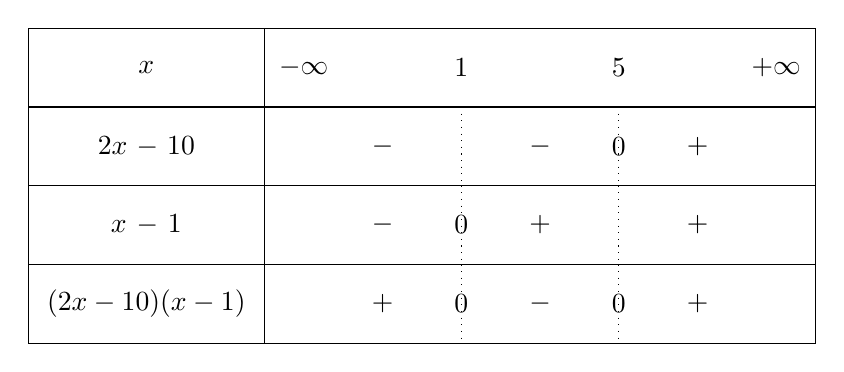
\begin{tikzpicture}
            \tkzTabInit[lgt=3,espcl=2]
            {$x$ /1,
              $2x-10$ /1,
            $x-1$ /1,
            $(2x-10)(x-1)$ /1}
            {$-\infty$,$1$,$5$,$+\infty$}%
            \tkzTabLine { ,-,t,-,z,+ }
            \tkzTabLine { ,-,z,+,t,+ }
            \tkzTabLine { ,+,z,-,z,+ }
          \end{tikzpicture}

      Les solutions se lisens dans la dernière ligne : $x\in]-\infty;1]\cup[5;+\infty[$.
  \end{enumerate}
\end{exercice}

\begin{exercice}[Développement, factorisation]~

  Soit $A(x)=(x+1)^2-(x+1)(2x-4)$, avec $x\in{\mathbb R}$.
  \begin{enumerate}
    \item \emph{Développer, réduire et ordonner $A(x)$.}\\
      $A(x)=x^2+2x+1-(2x^2-4x+2x-4)$\\
      $A(x)=-x^2+4x+5$
    \item \emph{Factoriser $A(x)$.} On repart de la première expression.\\
      $A(x)=(x+1)[(x+1)-(2x-4)]$\\
      $A(x)=(x+1)(x+1-2x+4)$\\
      $A(x)=(x+1)(-x+5)$
    \item \emph{Choisir la forme la plus adaptée pour résoudre dans $\mathbb R$ les équations suivantes.}

      \begin{multicols}{2}
      \begin{enumerate}
      \item On part de la forme factorisée :\\
        $(x+1)(-x+5)=0$\\
        donc $x+1=0$ ou $-x+5=0$, c'est-à-dire $x=-1$ ou $x=5$.
      \item On part de l'expression développée.\\
        $-x^2+4x+5=5$\\
        $-x^2+4x=0$\\
        $x(-x+4)=0$\\
        $x=0$ ou $-x+4=0$\\
        $x=0$ ou $x=4$
      \item On part de l'expression de départ.\\
        $(x+1)^2-(x+1)(2x-4)=(x+1)^2$\\
        $-(x+1)(2x-4)=0$\\
        $(x+1)(2x-4)=0$\\
        $x+1=0$ ou $2x-4=0$\\
        $x--1$ ou $x=2$
      \end{enumerate}
    \end{multicols}
  \end{enumerate}
\end{exercice}

\begin{exercice}[Repérage]~

  Soient les points $A(-1;1)$, $B(2;3)$, $C(4;2)$, $D(1;0)$.
  \begin{enumerate}
    \item \emph{Placer ces points dans un repère orthonormé.}

      \begin{tikzpicture}
        \draw[dotted] (-2,-1) grid (5,4);
        \draw (-2,0) -- (5,0);
        \draw (0,-1) -- (0,4);
        \draw[->] (0,0) -- (1,0) node[midway,above]{$\vecteur\jmath$};
        \draw[->] (0,0) -- (0,1) node[midway,left]{$\vecteur\imath$};
        \draw (-1,1) node{$\bullet$} node[below left]{$A$};
        \draw (2,3) node{$\bullet$} node[below left]{$B$};
        \draw (4,2) node{$\bullet$} node[below left]{$C$};
        \draw (1,0) node{$\bullet$} node[below left]{$D$};
      \end{tikzpicture}
    \item On va déterminer de deux manières différentes la nature du quadrilatère $ABCD$.
      \begin{description}
        \item[(a)] $\vecteur{AB}\coord{x_B-x_A}{y_B-y_A}$ donc
          $\vecteur{AB}\coord{2-(-1)}{3-1}$, soit 
          $\vecteur{AB}\coord{3}{2}$.
                   
                   De même, $\vecteur{DC}\coord{x_C-x_D}{y_C-y_D}$ donc
                   $\vecteur{DC}\coord{4-1}{2-0}$ donc
                   $\vecteur{DC}\coord{3}{2}$.

                   Les deux vecteurs sont égaux, donc $ABCD$ est un parallélogramme.
                 \item[(b)] Soit $I({x_I},{y_I})$ le milieu de $[AC]$. Alors 
                   $x_I=\frac{x_A+x_C}{2}=\frac{-1+4}{2}=\frac{3}{2}$,
                   et $y_I=\frac{y_A+y_C}{2}=\frac{ 1+2}{2}=\frac{3}{2}$ : $I(\frac{3}{2},\frac{3}{2})$.

                   De même, les coordonnée du milieu de $[AD]$ sont $({\frac{3}{2}},{\frac{3}{2}})$.

                   $ABCD$ est donc un quadrilatère qui a ses diagonales se coupant en leur milieu : c'est un parallélogramme.
      \end{description}
    \item Pour savoir si $ABCD$ est un losange, une des méthodes est de calculer la longueur de deux côtés consécutifs.
      \begin{itemize}[$\bullet$]
        \item $AB=\sqrt{(x_B-x_A)^2+(y_B-y_A)^2}=\sqrt{(2-(-1))^2+(3-1)^2}=\sqrt{3^2+2^2}=\sqrt{13}$.
        \item $BC=\sqrt{(x_C-x_B)^2+(y_C-y_B)^2}=\sqrt{2^2+(-1)^2}=\sqrt{5}$.
      \end{itemize}
      Donc $AB\neq BC$ : $ABCD$ n'est pas un losange.
  \end{enumerate}
\end{exercice}

\begin{exercice}[Repérage, algorithmique]~
  \begin{enumerate}
    \item Voir le cours.
    \item \begin{enumerate}
    \item L'algorithme vérifie si le triangle dont les coordonnées sont données en entrée est rectangle ou non. Il affiche Vrai si c'est le cas, et Faux sinon.
    \item Solution :
      \begin{lstlisting}[language=naturel,frame=lines,mathescape=true,numbers=left]
      Lire $x_A$
      Lire $y_A$
      Lire $x_B$
      Lire $y_B$
      Lire $x_C$
      Lire $y_C$
      $\sqrt{(x_B-x_A)^2+(y_B-y_A)^2}$ -> $AB$
      $\sqrt{(x_C-x_A)^2+(y_C-y_A)^2}$ -> $AC$
      Si AB=AC
      Alors
        Afficher "Vrai"
      Sinon
        Afficher "Faux"
      FinSi
      \end{lstlisting}
      \end{enumerate}
  \end{enumerate}

\end{exercice}

\end{document}
